\documentclass[a4paper,10pt]{article}
\usepackage[utf8x]{inputenc}
\usepackage{graphicx}
%opening
\title{Cartesian Cut Cell Grid Generator}
\author{Bruce Duncan}

\begin{document}

\maketitle

\section{Introduction}

This software implements the Cut Cell method as described by \cite{dingram}. It
is intended to provide a computation mesh for the simulation of the flow around
solid bodies in Code\_Saturne \cite{code_saturne}.

\section{Method}

The cut cell method produces a computational mesh which is mostly Cartesian
except where Cartesian cells intersect the solid, where the mesh is
tetrahedral. To achieve this, the library creates a background grid of unit
cubes at each point in three dimensions. It then computes the intersection of
each of these cubes with the solid and proceeds based on the output:
\begin{itemize}
 \item If the result contains no points, then the cube is completely inside the
solid and no processing is required,
\item If the result contains only the eight points of the original cube, then
the cube is completely outside the solid and will be processed as a fluid cell,
and,
\item If the result is neither of these, the cell must be cut to fit the
boundary of the solid.
\end{itemize}

The latter case, which involves computing the tetrahedral mesh of the cut cells,
is the most interesting. For reasons which will become clear in the next
section, we decompose the resulting polyhedron of each cell into many convex
polyhedra. These polyhedra are then further decomposed into tetrahedra before
being output.

\begin{figure}[htb]
 \centering
 \includegraphics[width=\textwidth,keepaspectratio=true]{./cutcellplot.pdf}
 % cutcellplot.pdf: 794x687 pixel, 96dpi, 21.01x18.17 cm, bb=0 0 595 515
 \caption{Example grid showing fluid and cut cells.}
 \label{fig:plot}
\end{figure}

An example of the generated fluid and cut cells is shown in
Figure~\ref{fig:plot}. There also exists a single solid cell at the origin.

\section{Implementation}

The software uses the Computational Geometry Algorithms Library (CGAL)
\cite{cgal}, which is a C++ library which uses templates to provide different
behaviour through various number ``kernels''. It provides ``Nef\_polyhedra'', a
polyhedron whose structure is specified through a boundary representation
with a local sphere map description of vertices. A sphere map is a polyhedron of
dimension two which provides a complete representation of the boundary of the 3D
polyhedron. This representation is closed under boolean operations and we rely
on this to produce polyhedra which are not malformed. Polyhedra which are not
usable include those with two or more points representing a single vertex.

The ``cutcell'' program is written in C++ to allow easy integration with CGAL
and the CFD General Notation System (CGNS) \cite{cgns} C library, which is well
supported by Code\_Saturne.

The ``cutcell'' library and the command line interface use the Boost
\cite{boost} library to provide a 3-dimensional array and command line argument
processing.

\subsection{Structure}

This section gives an overview of the structure of the code. The files are
arranged as follows:

\begin{description}
 \item[CMakeLists.txt] CMake build rules
 \item[COPYING] Copyright statement
 \item[INSTALL] Installation instructions
 \item[cutcell.cpp] cutcell library
 \item[cutcell.ui] GUI MainWindow definition
 \item[cutcellcli.cpp] Command line interface to the library, using Boost
 \item[cutcellgui.cpp] Graphical user interface to the library, written in Qt
 \item[debian/] A set of files to control creation of a Debian package
 \item[include/cutcell.hpp] API to the library
 \item[include/cutcellgui.hpp] GUI definitions
 \item[make\_cube\_3.cpp] A program to create a unit cube, which is then stored
in include/cutcell.hpp.
\end{description}

The logical structure of the code consists of a \textit{Grid} class and a
\textit{Cell} class containing an enum called \textit{Type}. These are
described later.

\subsection{Library API}

The cutcell library exposes a \textit{Grid} class which performs the cutting.
The job of the user interfaces is to parse the input files, apply any
transformations and add them to the Grid object. The grid transformations are
then registered with the Grid object using \textit{addTransform} and the
cutting begins with a call to \textit{cut}.

To extract the resulting mesh, a number of methods are available.
\textit{ostream} operators are available, and a \textit{GridFormat} class
allows the stream being used to store the desired output format type. CGNS, VTK
and Nef output methods are provided, but the user interfaces only output CGNS.

An alternative method to output CGNS is provided which avoids having to write a
temporary file through the \textit{ostream} system. \textit{output\_cgns\_file}
outputs CGNS to the named file.

\subsection{Cutting algorithm}

This section details the operation of the cutcell library. Most of these
details are hidden from the drivers detailed in the previous section.

The Grid constructor creates a few internal object required for the cutting
process, such as the 3D arrays of Nef\_polyhedra and Cell objects (which store
the type of each cell). It also initialises the Nef\_polyhedra which represents
the solid, and the transformation which will be applied to the grid. These are
initialised to the empty set and the identity transform, respectively. A unit
cube at the origin is also initialised.

There are two methods which allow input into the Grid object. \textit{addSolid}
and \textit{addTransform} add the given Nef\_polyhedra and Aff\_transformation
objects to the internal objects.

The \textit{cut} function starts by computing the iso-oriented bounding box of
the solid. That is, the bounding box which has its boundaries coplanar with
each of the three axes, and therefore the boundaries of the fluid cells. This
allows the intersection test to be avoided if the cell in question is clearly
outside the solid.

For each of the cells in the grid, a copy of the unit cube is translated to the
same position as the cell. Then, a new Nef\_polyhedron is constructed which is
the intersection of this cube with the solid object. For this new polyhedron:
\begin{itemize}
 \item if it is the empty set, set the cell type to \textit{Solid},
 \item if it is equivalent to the test cube, set the cell type to
\textit{Fluid},
 \item otherwise, decompose the new Nef\_polyhedron into convex parts and store
it in the array. Set the cell type to \textit{Cut}.
\end{itemize}

The cutting is then complete. A user of the library may obtain the result using
the \textit{grid} and \textit{cell} functions, which return a 3D array of
Nef\_polyhedra and Cell objects, respectively. Alternatively, as is done with
the cutcell command-line program and the GUI, one may use the CGNS output
detailed next.

\subsection{CGNS output}

CGNS is well-supported by Code\_Saturne and provides many 3D polyhedra to
represent the computational domain. We use the \textit{HEXA\_8} and
\textit{TETRA\_4} 3D elements to represent the grid. HEXA\_8 is a cuboid in 3D
space with eight points. TETRA\_4 is a tetrahedron with four points. We use
QUAD\_4 elements to represent the 2D boundary elements on the exterior
boundary. We use TRI\_3 elements to represent the 2D boundary with the
tetrahedra of the solid between the cut cells and the solid cells.

CGNS separately stores the 3D coordinates of the vertices and the edges which
make up the polyhedra. The points are stored as a list of double precision
numbers in three \textit{GridCoordinates} nodes each with a special name like
``CoordinateX''. The elements which refer to them are a list of the indices
into the GridCoordinate sections in an \textit{Elements} node. There is one
Elements section for each type of polyhedron.

In order to output the CGNS, we loop over all cells in the grid. If the cell is
Fluid we make a simplification by explicitly generating each vertex of the
cube. This makes it much easier to output the vertices in the order defined by
CGNS. The eight vertex indices are transformed according to the input added to
the list which makes up the HEXA\_8 Elements node.

For a cut cell, some more processing is required. The cell has already been
converted to one or more convex polyhedra by the cutting algorithm. In order to
create tetrahedra, we use the CGAL Delaunay\_triangulation\_3 package which
creates a set of tetrahedral cells given a list of points. These points are
transformed, as for a fluid cell, and added to a separate list of TETRA\_4
nodes. We then store the Delaunay\_triangulation of each convex part of the
cell, so that we can output the boundary elements later.

At this point we have a complete description of the geometry of the grid, so we
write out the grid coordinates and the cuboid and tetrahedral volume sections to
the CGNS file. This provides an opportunity to free the memory used for volume
elements, although this is not done at present. We could stop here, but for ease
of use, we create boundary element sections. This involves iterating over all
cells on a boundary and performing a similar function as for the volume
elements. As before, the rectangle on each boundary is created manually and the
four points are transformed and added to a list. For the triangles, we iterate
over all tetrahedra, outputting three points if exactly three points of the
tetrahedron lie on the plane of the boundary. We write CGNS boundary conditions
as each of the six boundaries is processed. This gives the boundary a
convenient name, for example, ``IloFluid'' for the Fluid boundary at the
boundary in the $yz$-plane nearest the origin.

\subsection{Command Line Interface}

The CLI is a simple C++ program which collects command line arguments, arranges
for input and output files and calls the cutcell library to produce CGNS output.

\subsection{Graphical User Interface}

The GUI is a Qt \cite{qt} C++ program which provides an easy method for users
to input various parameters and receive feedback about the gridding operation.
The main window was created in Qt designer and the result is in
\texttt{cutcell.ui}. This is processed in the build by moc to create
\texttt{include/moc\_cutcellgui.cxx}. The main program then includes this file
and can easily create an object which represents the GUI window. The GUI is a
fairly self-explanatory application, except for to note that the cutting is
done a separate \textit{GenerateThread} which makes the calls to the cutcell
library without interrupting the GUI. Errors and completion signals are passed
back to the GUI by use of a signal. This avoids the need for explicit locking.

\section{Usage Instructions}

\subsection{Getting the source}

The source may be obtained as a tarball from the author. It is also hosted on
github at http://github.com/bduncan/cutcell, along with the commit history of
the project and a bug tracker.

\subsection{Building}

The source tree includes an \texttt{INSTALL} file which gives simple
instructions for building the program from source and building a Debian
package.

To build the program, one must obtain and install the prerequisites, especially:

\begin{itemize}
 \item A C++ compiler. The project was tested with GCC 4.5.
 \item CMake. The project requires at least version 2.4.5 and was tested with
version 2.8.3.
 \item The Boost C++ library packages \textit{program\_options} and
\textit{multi\_array}. The project was tested with version 1.42.
 \item The CGAL library. The project was tested with CGAL 3.7 and 3.8. Earlier
versions are known to cause problems.
 \item The CGNS library. The project was tested with version 2.5.4.
 \item The Qt library for building the GUI. The project was tested with
version 4.7.2.
\end{itemize}

All of these packages are available in modern Linux package managers.

To set up the build environment, \textit{cmake-gui} provides an easy method to
specify the location of the necessary libraries. Once CMake has generated the
build files, one should be able to run \texttt{make} to create the executables.

\subsection{Running}

\begin{figure}[htb]
 \centering
 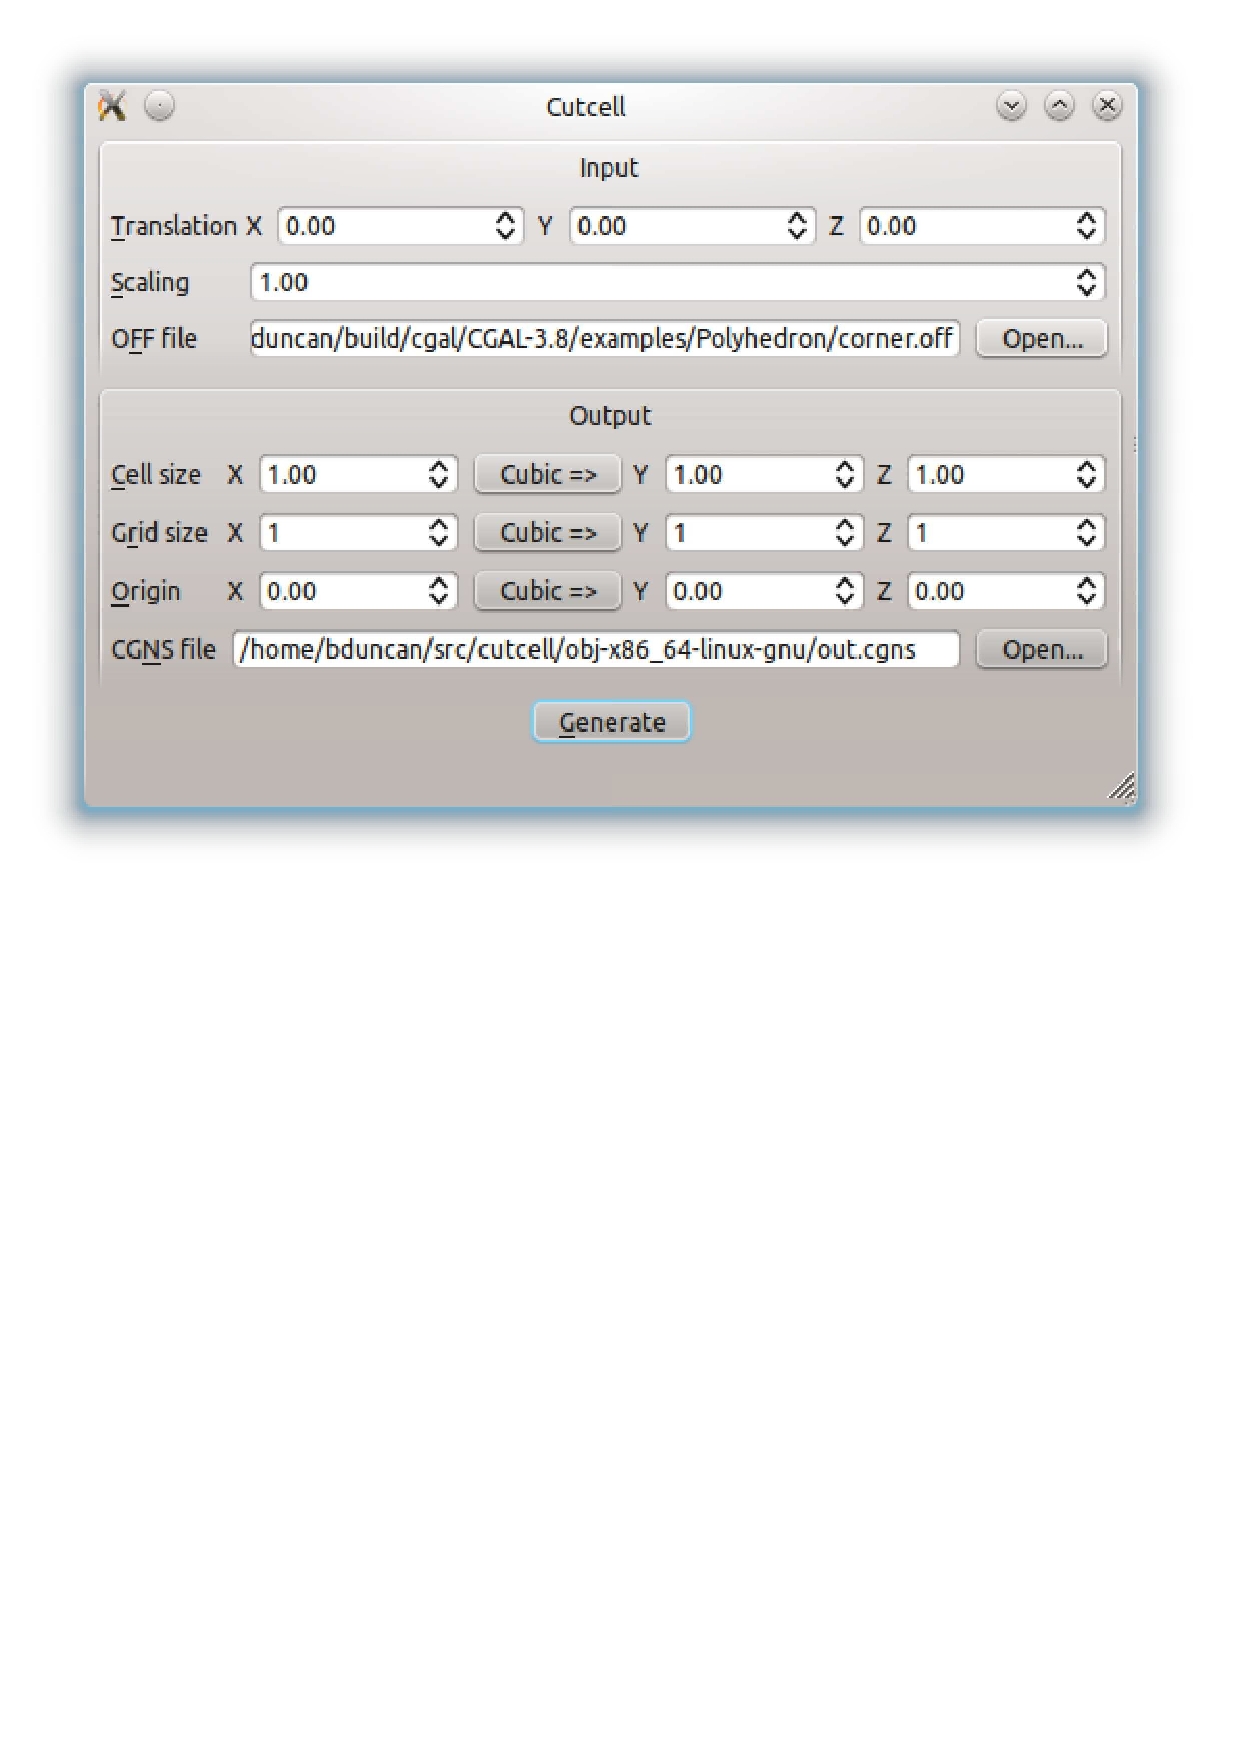
\includegraphics[keepaspectratio=true,width=\textwidth]{./cutcellgui.pdf}
 % cutcellgui.pdf: 595x842 pixel, 72dpi, 20.99x29.70 cm, bb=0 0 595 842
 \caption{The cutcell GUI}
 \label{fig:gui}
\end{figure}

The software consists of two user interfaces to the library, one Graphical User
Interface (GUI) shown in Figure~\ref{fig:gui} and one Command Line Interface
(CLI). Both allow the user to convert a polyhedral surface in Object File Format
(OFF) to a CGNS mesh. Both allow the user to specify scaling and translation
parameters for the input solid, and allow a grid size, cell size and origin to
be specified.

In using the GUI, the user is presented with default values for the position of
the input solid and the properties of the grid, these being zero or one as
appropriate. The position and size of the input solid may be specified as a
translation vector and a scale factor in three dimensions. The output CGNS grid
may have an arbitrary cell size in three dimensions, an integer number of grid
cells in each dimension and an arbitrary translation vector for the origin.

To use the CLI, the user must specify only the size of the grid. Other
parameters assume reasonable defaults and the program reads an OFF file from
standard input, writing a CGNS file on standard output. Errors messages, and
debugging, if configured, are written on standard error.

\section{Examples}

\subsection{Airfoil}

We create an airfoil using Xfoil \cite{xfoil}, transform the 2D coordinates into
a 3D solid and cut it using our algorithm. We then import the grid into
Code\_Saturne.

First, open Xfoil. Select a NACA 0012 airfoil by entering \texttt{NACA 0012}. To
generate a reasonable size grid, we reduce the number of points being used. Open
the panelling parameters menu by typing \texttt{ppar} \footnote{This opens
another window showing the buffer, experience suggests that closing this window
will cause a crash.}. Alter the number of panel nodes by typing \texttt{n} and
entering \texttt{40}. Output the grid by typing \texttt{psav out.off}.

Next, we convert this 2D grid into a 3D solid. This can be done by hand or by
using the supplied \texttt{3dairfoil.py} program. We use the python program as
a filter: \texttt{3dairfoil.py < out.off > airfoil.off}.

At this point, we can confirm that the airfoil is output as expected by reading
it in a program such as geomview \cite{geomview}.

Next, the generated OFF file is supplied to the cutcell program. We want to
generate a large enough grid to produce a meaningful simulation, so we use a
grid of size $120 x 60 x 40$. We place the airfoil at roughly the centre of the
domain by applying an offset of $40 x 30 x 0$. We want an airfoil such that
there is approximately one airfoil point per grid point, so apply a scale
factor of $40$:

\begin{verbatim}
cutcell -I ../airfoil_40_3d.off -O out.cgns
-X 120 -Y 60 -Z 40
-x 40 -y 30
--scaling 40
\end{verbatim}

Once the gridding is complete, we can check the CGNS output using the adfviewer
and cgnsplot tools provided with CGNS.

\bibliographystyle{plain}
\bibliography{report}

\end{document}
